\section{Lighting and Shading}

In lighting we have to differentiate between local and global illumination models. Local illumination models only consider the direct interaction of a light source with an object surface, the global illumination model also considers indirect lighting. We mostly focus on local illumination models.


\subsection{Measuring Light}

Radiometry is the study of measuring electromagnetic radiation, including visible light. We first introduce some definitions:
\begin{itemize}
	\item \textbf{Angle} - $\theta = \frac{l}{r}$, for a circle $2 \pi$ radians
	\item \textbf{Solid Angle} - $\Omega = \frac{A}{r^2}$, for a sphere $4 \pi$ steradians
	\item \textbf{Direction} - point on the unit sphere parameterized by two angles $\omega = (\theta, \phi)$ (zenith and azimuth)
\end{itemize}

\begin{center}
	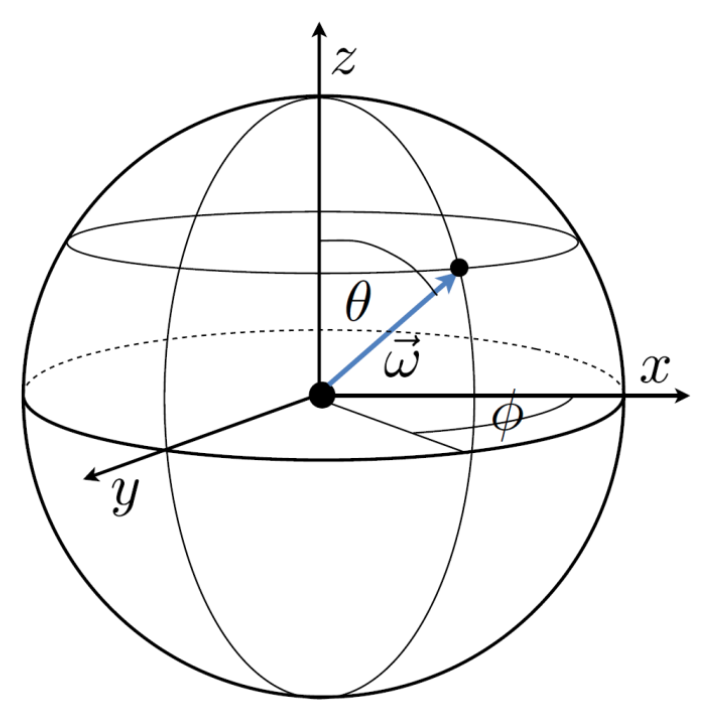
\includegraphics[width=0.5\linewidth]{unit_sphere.png}
\end{center}

Now we can define light as consisting of photons with a position $x$, a direction $\omega$ and a wavelength $\lambda$. Each photon has an energy of $hc / \lambda$. \medskip

The basic quantities to measure light are then defines as:
\begin{itemize}
	\item \textbf{Flux} $\Phi$ - total amount of energy passing through a surface or space per time unit
	\item \textbf{Irradiance} $E$ - flux per unit area arriving at a surface 
	\item \textbf{Radiosity} $B$ - flux per unit area leaving a surface 
	\item \textbf{Intensity} $I$ - flux per solid angle 
	\item \textbf{Radiance} $L$ - intensity per unit area or flux density per unit solid angle 
\end{itemize}
\begin{center}
	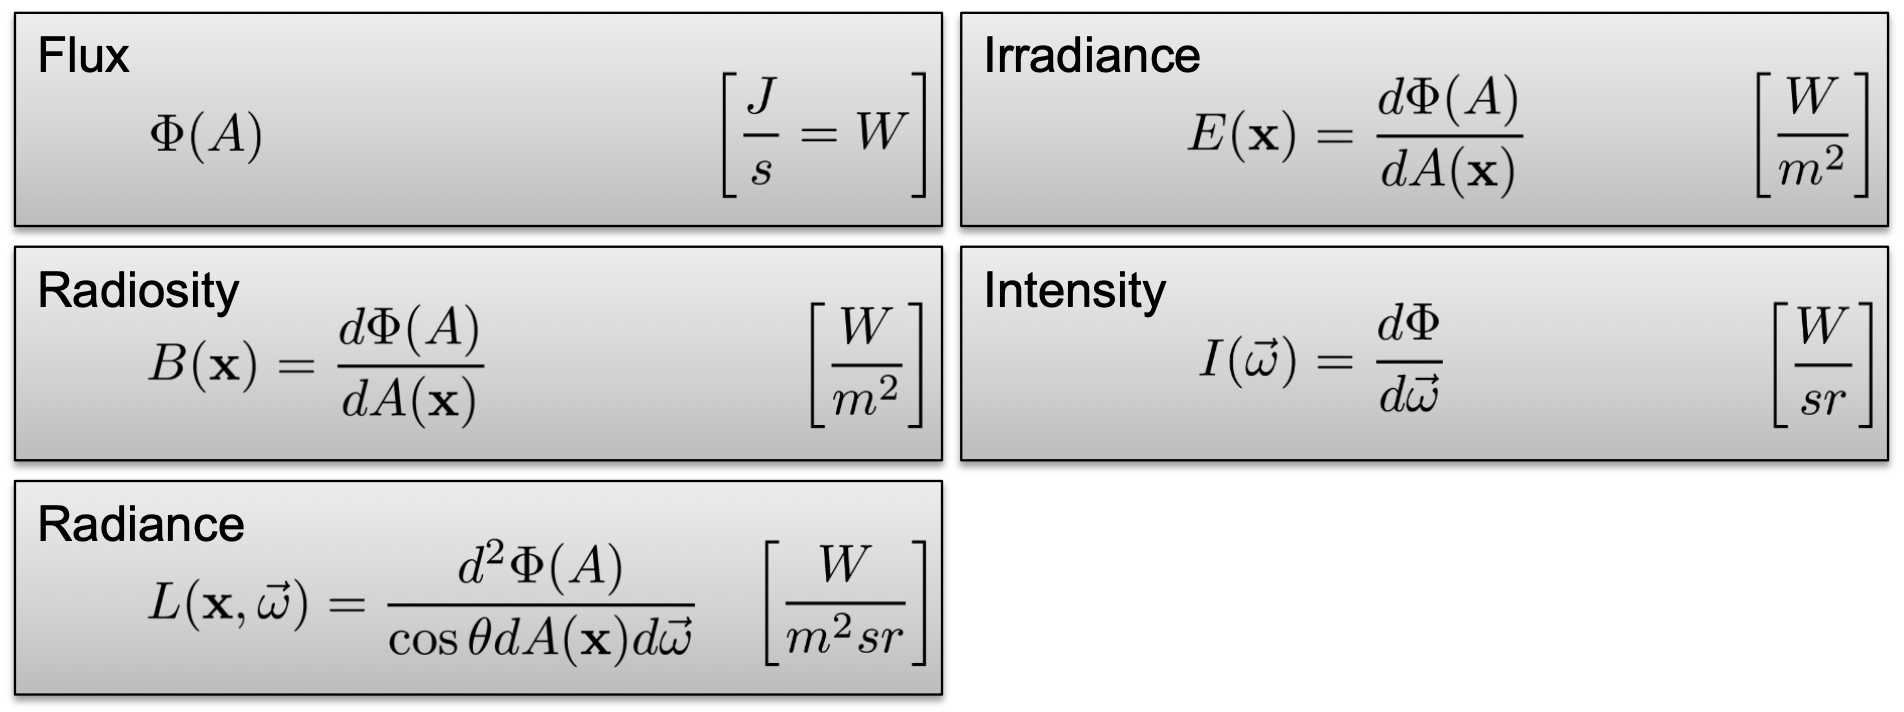
\includegraphics[width=\linewidth]{radiometry.png}
\end{center}


\subsection{Reflection Models}

\subsubsection{BRDF}

Bidirectional Reflectance Distribution Function (BRDF) models the surface and its reflection of light. The BRDF provides a relation between incident radiance and differential reflected radiance.
$$f_r(x, \omega_i, \omega_r) = \frac{dL_r(x, \omega_r)}{L_i(x, \omega_i) \cos \theta_i d \omega_i}$$

From this we can derive the \textbf{reflection equation}:
$$L_r(x, \omega_r) = \int_{H^2} f_r(x, \omega_i, \omega_r) L_i(x, \omega_i) \cos \theta_i d \omega_i$$

The reflection equation describes a local illumination model. BRDF has the ability to express a large variety of complex materials. There are large libraries of measured BRDFs for different materials.

\subsubsection{Simpler Reflections}

These physical based models where for a long time to complex, so a simpler model was used. A material was characterized by a combination of diffuse and specular reflexion.
\begin{center}
	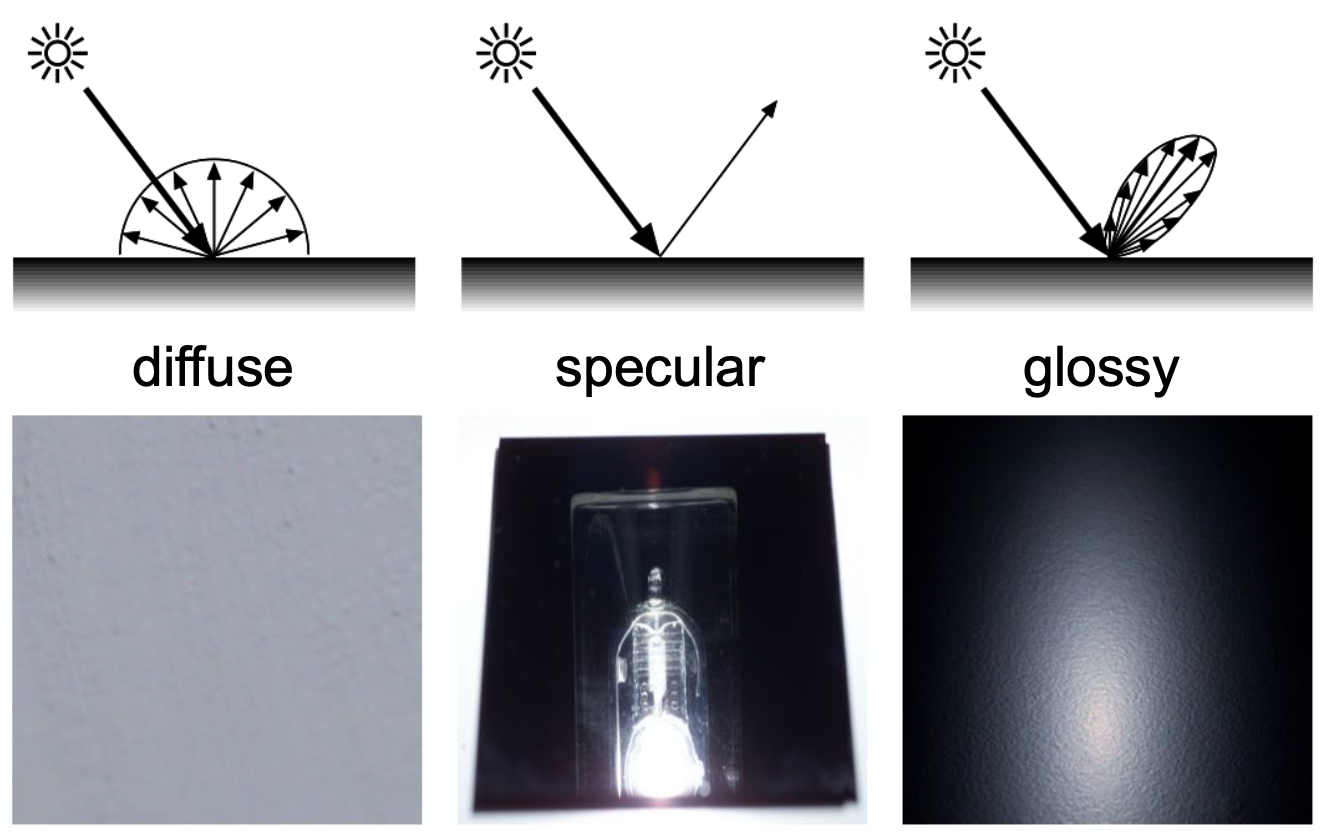
\includegraphics[width=\linewidth]{reflections.png}
\end{center}

For diffuse reflection, the BRDF is a constant, since it is the same value over the whole hemisphere.
$$L_r(x) = f_r E_i(x)$$

\subsubsection{Phong Illumination}

OpenGL uses simplified reflections, one of the most used models is the phong illumination model. \medskip

\textbf{Ambient Light} comes from all directions. Its reflection is independent of the cameras position, light position and surface orientation. So we can model the reflection intensity by using a light source and a material parameter.
$$I = I_a k_a$$

\textbf{Diffuse Reflection} is dependent on directed light $I_p$ (light source position) and the orientation of the source. It still is independent of the camera position. So we can model the reflection intensity by either using a cosine or the dot product using the surface normal.
$$I = I_p k_d \cos \theta = I_p k_d (N \cdot L)$$

In a very simple model, we can now simply take the sum of the ambient light and the diffuse reflection. 
$$I = I_a k_a + I_p k_d (N \cdot L)$$

To improve on this we can add quadratic attenuation due to spatial radiation (quadratically less energy when moving away from the source).
$$I = I_a k_a + f_{att} I_p k_d (N \cdot L) \qquad f_{att} = \frac{1}{d_L^2}$$

To further improve we can add the specular reflection. This depends on the angle between the reflection $R$ and viewing ray $V$.
\begin{center}
	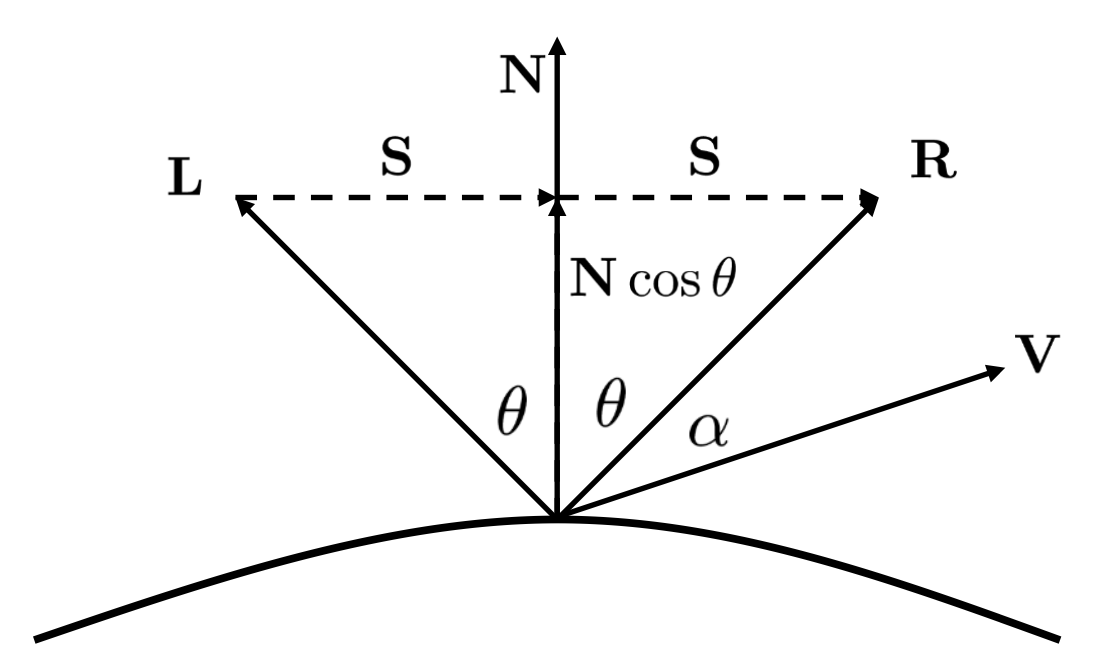
\includegraphics[width=0.7\linewidth]{specular_reflection.png}
\end{center}

Combining this we end up with a simple but already quite good model for lighting.
\begin{center}
	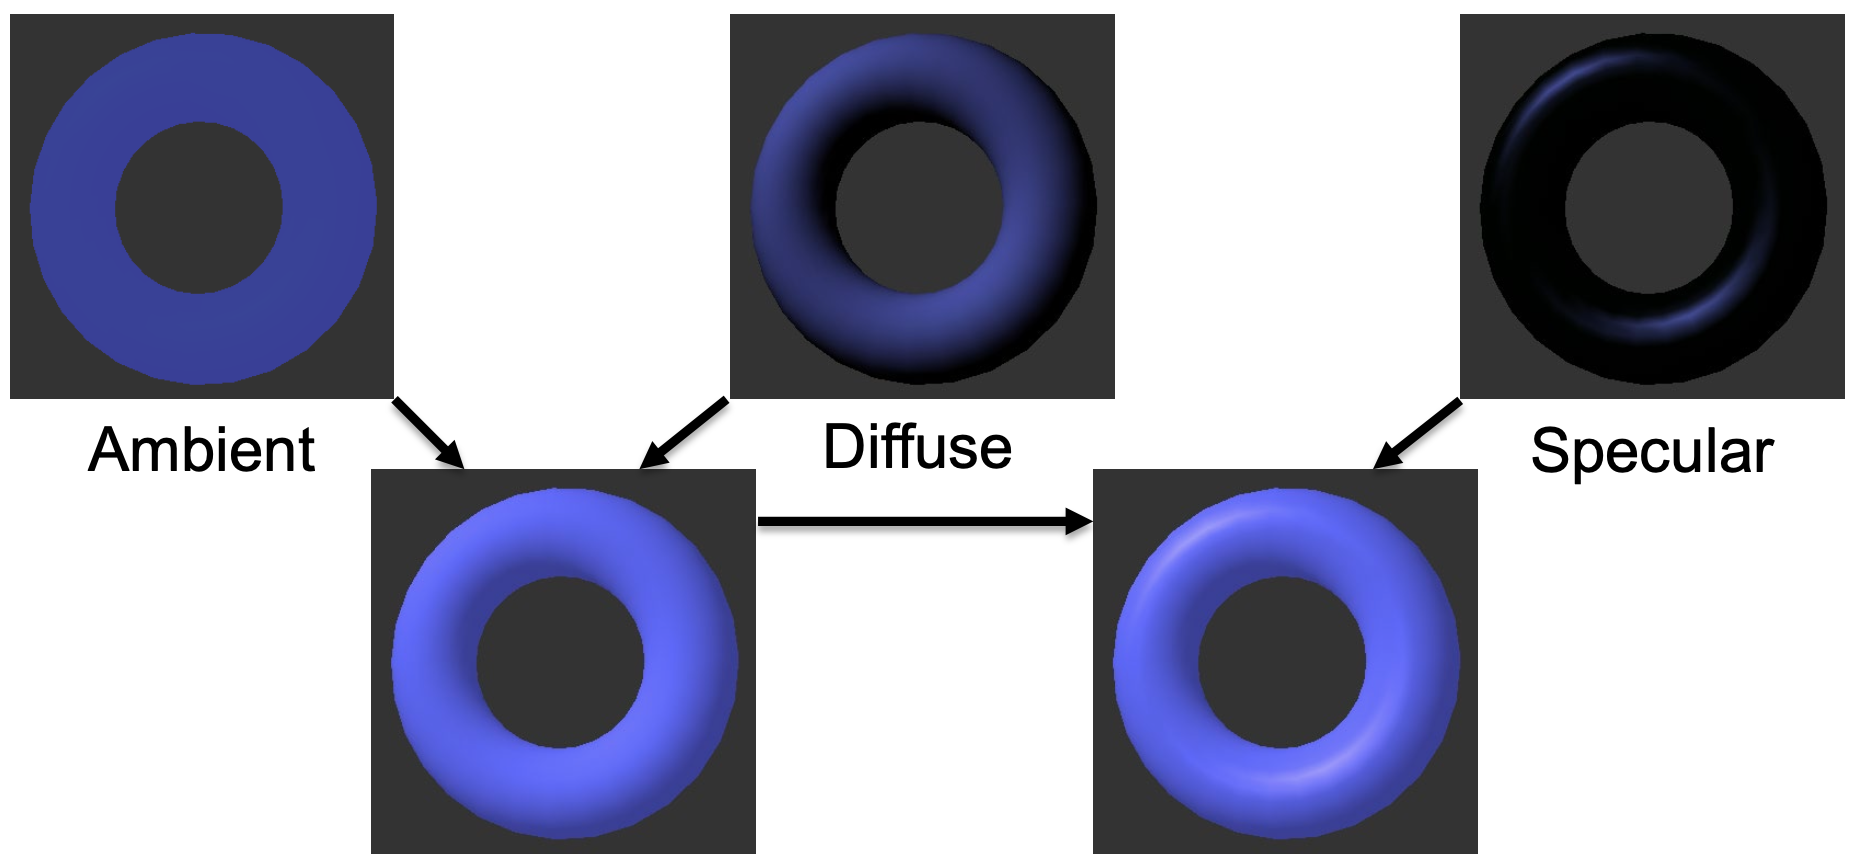
\includegraphics[width=\linewidth]{lighting_model.png}
\end{center}

The phong illumination model approximates specular reflection by cosine powers. It also makes the whole function dependent on the wavelength.
$$I_\lambda = I_{a \lambda} k_a O_{d \lambda} + f_{att} I_{p \lambda} [k_d O_{d \lambda}(N \cdot L) + k_s (R \cdot V)^n]$$


\subsection{Shading Models}

We have seen how to calculate the lighting of an object, now we want to know how to calculate the color per primitive. The simplest model would be to have a single color per primitive, this is called flat shading and happens in screen space. This does not look good as a primitive converts to many pixels.

\subsubsection{Gouraud Shading}

Similar to flat shading, gouraud shading also happens in screen space. It works by calculating the face normals and then the vertex normals by averaging the face normals. After that we evaluate illumination for each vertex and then interpolate the vertex colors bilinearly on the current scan line.
\begin{center}
	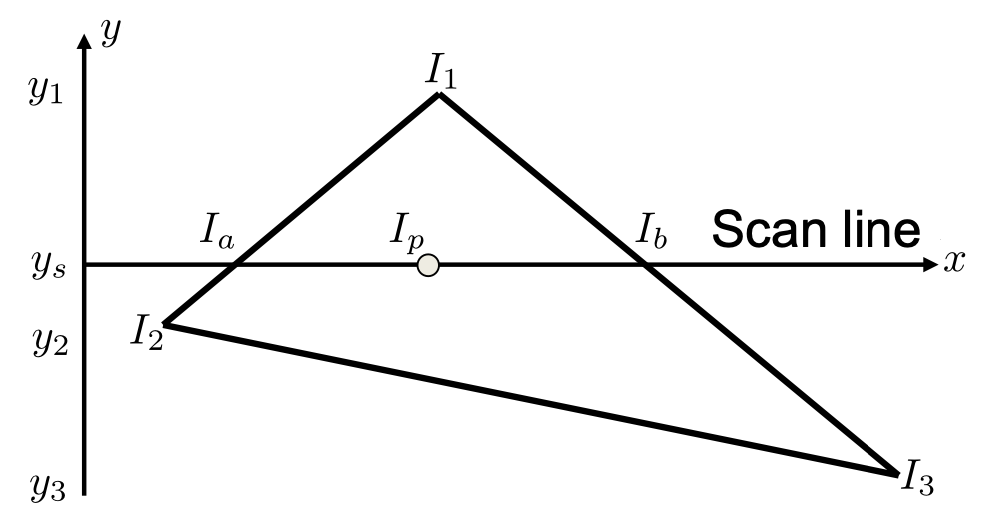
\includegraphics[width=0.7\linewidth]{gouraud_scanline.png}
\end{center}

There are a few problems with scan line interpolation. The first one being perspective distortion, as we interpolate in the projection plane. Further the interpolation is orientation dependent and quality depends on the size of primitives.

\subsection{Phong Shading}

Phong shading happens in object space. It works by barycentric interpolation of the surface normals. The color is then determined by the interpolated normal.
\begin{center}
	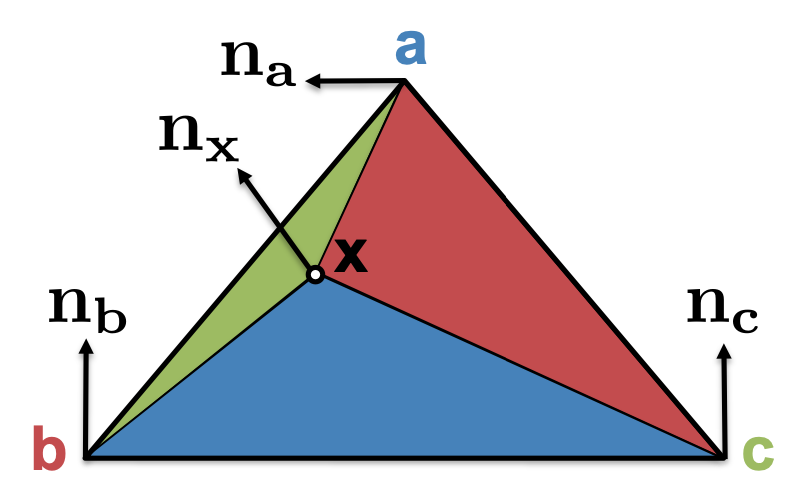
\includegraphics[width=0.7\linewidth]{phong_interpolation.png}
\end{center}

Phong shading cannot be applied if the normal is not defined.

\subsection{Transparency}

The typical color format includes an alpha channel, indicating the level of transparency. If we have partially transparent object, we need to blend the colors of the different objects together. One approach for this is \textbf{alpha blending}.
\begin{center}
	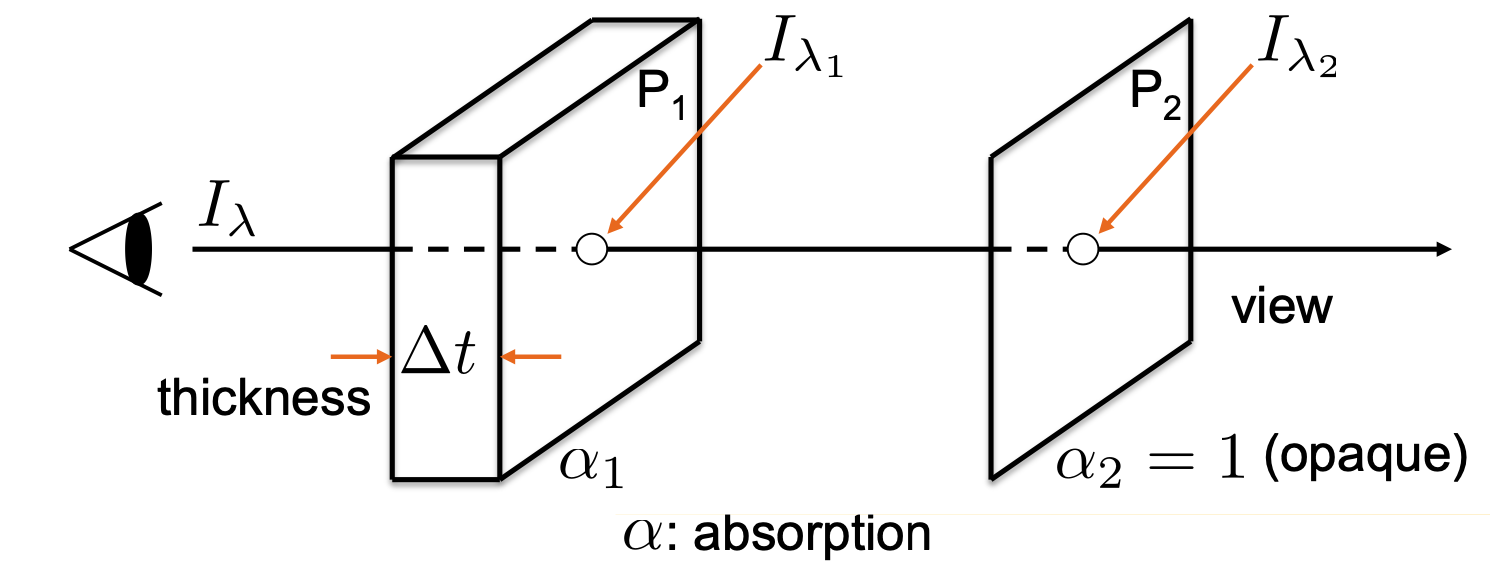
\includegraphics[width=\linewidth]{alpha_blending.png}
\end{center}

The intensity of the opaque object gets filtered by the object in front of it.
$$I_\lambda = I_{\lambda_1} \alpha_1 \Delta t + I_{\lambda_2} e^{- \alpha_1 \Delta t} \approx I_{\lambda_1} \alpha_1 + I_{\lambda_2} (1- \alpha_1)$$

To evaluate the alpha blending, we need to have an order to the primitives. This is the reason that we store the distance even in the screen space representation. Having that distance value (z-buffering) allows us to apply \textbf{back to front rendering} of the primitives. However this does not work anymore if we have intersecting objects. \medskip

To solve this problem we use \textbf{depth peeling}. It works by using multiple passes, each pass renders the next closest fragment.



















